% asset_id: AS2ModellingInMechanicsTIKZ-005
\documentclass[tikz,border=8pt]{standalone}
\usepackage{amsmath}
\usetikzlibrary{arrows.meta}
\begin{document}
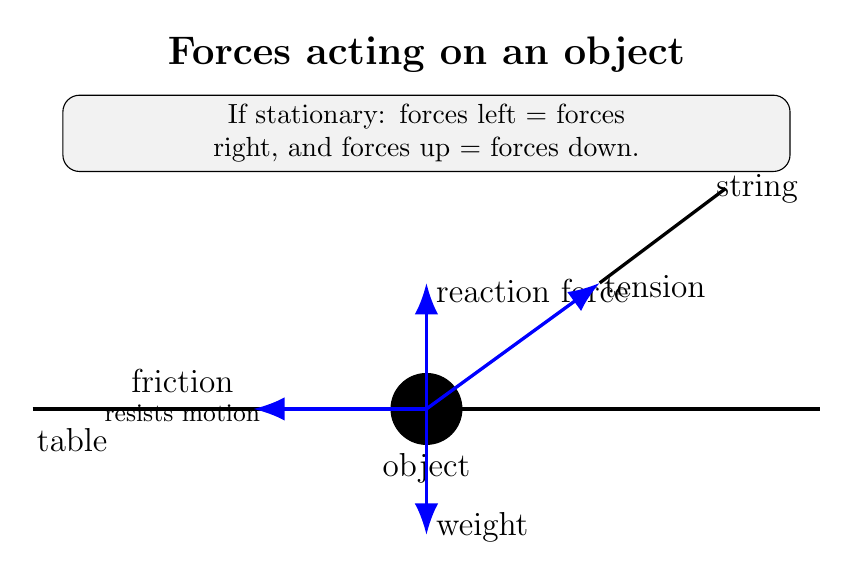
\begin{tikzpicture}[force/.style={-{Latex[length=4mm]}, very thick, blue}, label/.style={font=\large}]
\node[font=\Large\bfseries] at (0,4) {Forces acting on an object};\draw[very thick] (-5,-0.5) -- (5,-0.5);\node[label] at (-4.5,-0.9) {table};\filldraw[black] (0,-0.5) circle (0.45);\node[label] at (0,-1.25) {object};
\draw[force] (0,-0.5) -- (0,-2.1);\node[label, right] at (0,-2.0) {weight};\draw[force] (0,-0.5) -- (0,1.1);\node[label, right] at (0,1.0) {reaction force};\draw[force] (0,-0.5) -- (-2.2,-0.5);\node[label] at (-3.1,-0.15) {friction};\node[font=\small] at (-3.1,-0.55) {resists motion};\draw[force] (0,-0.5) -- (2.2,1.1);\draw[very thick] (2.2,1.1) -- (3.8,2.3);\node[label] at (2.9,1.05) {tension};\node[label] at (4.2,2.3) {string};\node[draw, rounded corners=6pt, align=center, fill=gray!10, text width=9cm] at (0,3.0) {If stationary: forces left = forces right, and forces up = forces down.};
\end{tikzpicture}
\end{document}
